\chapter{PCLc}

\section{Syntax}
\begin{figure}[!h]
  \centering
    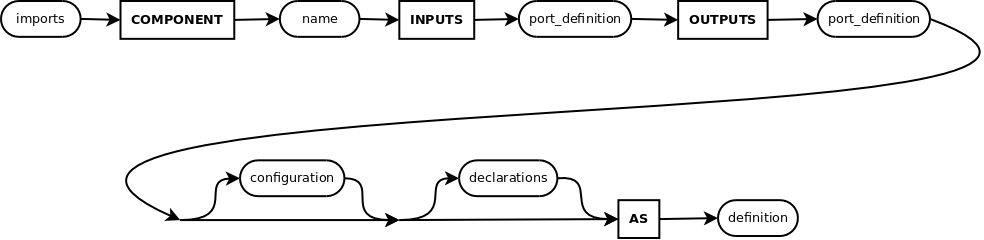
\includegraphics[width=1.0\textwidth]{chapters/compiler/diagrams/pcl-top-level}
  \caption{PCL file syntax.}
  \label{fig:pcl-top-level}
\end{figure}

\subsection{Imports}
\begin{figure}[!h]
  \centering
    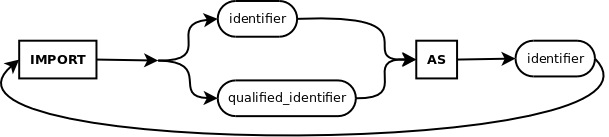
\includegraphics[width=1.0\textwidth]{chapters/compiler/diagrams/pcl-imports}
  \caption{Importing PCL files.}
  \label{fig:pcl-imports}
\end{figure}

\subsection{Port Definitions}
\begin{figure}[!h]
  \centering
    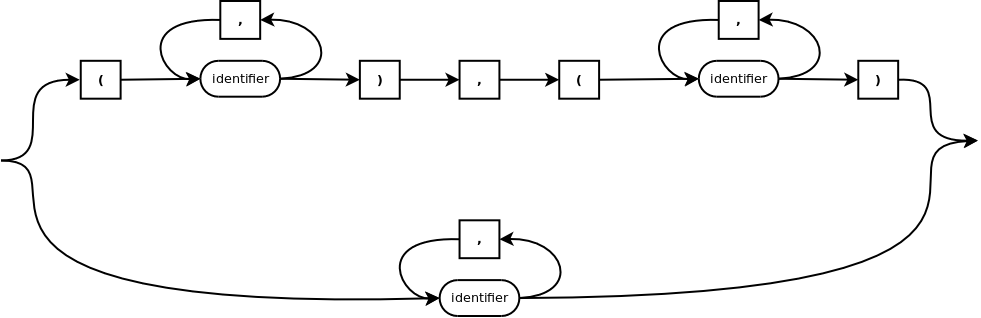
\includegraphics[width=1.0\textwidth]{chapters/compiler/diagrams/pcl-port-defs}
  \caption{Component Port Definition.}
  \label{fig:pcl-port-defs}
\end{figure}

\subsection{Configuration}
\begin{figure}[!h]
  \centering
    \includegraphics[width=1.0\textwidth]{chapters/compiler/diagrams/pcl-config}
  \caption{Component Configuraton.}
  \label{fig:pcl-config}
\end{figure}

\subsection{Declarations}

\subsection{Definition}
